\documentclass{article}

% Required packages
\usepackage{amssymb}
\usepackage{amsmath}
\usepackage{graphicx}
\usepackage{geometry}
\usepackage{tikz}
\usepackage{array}
\usepackage{booktabs}
\usepackage{enumitem}
\usepackage{listings}
\usepackage{xcolor}
\usepackage{fancyhdr}
\usepackage{float}
\usepackage{subcaption}
\usepackage{comment}

% Set page geometry
\geometry{a4paper, margin=1in}

% Configure listings for Python
\lstset{
  language=Python,
  basicstyle=\ttfamily\footnotesize,
  numbers=left,
  numberstyle=\tiny\color{gray},
  frame=single,
  breaklines=true,
  breakatwhitespace=true,
  captionpos=b,
  tabsize=4,
  showspaces=false,
  showstringspaces=false,
  showtabs=false,
  commentstyle=\color{gray}\textit,
  keywordstyle=\color{blue}\bfseries,
  stringstyle=\color{red}
}

\begin{document}

\pagestyle{fancy}
\chead{DSC 257: Unsupervised Learning (Fall 2025)}
\lhead{Homework 11}
\rhead{Randall Rogers}

%------------------
% Solution for 1(a) and 1(b)
%------------------
\subsection*{Solution 1}
\noindent\rule{\textwidth}{0.4pt}\\

\subsubsection*{Solution 1 (a)}
\subsubsection*{Step 1: Identify characteristics of the dataspace}
\parbox{\textwidth}{
We are given 10 dimensional vectors where each element can be any real number ($x_{i} \in \mathbb{R}$):
}


\subsubsection*{\normalfont}{$\therefore$ we can express the dataspace $\chi$ as: $\chi = \mathbb{R}^{10}$}

\noindent\rule{\textwidth}{0.4pt}\\

\subsubsection*{Solution 1 (b)}
\subsubsection*{Step 1: Identify characteristics of the dataspace}
\parbox{\textwidth}{
We are given 3 dimensional vectors where each element is zero or one ($x_{i} \in [0,1]$):
}

\subsubsection*{\normalfont}{$\therefore$ we can express the dataspace $\chi$ as: $\chi = {[0,1]}^{3}$}

\noindent\rule{\textwidth}{0.4pt}\\

\newpage

%------------------
% Solution for 2(a),2(b), and 2(c)
%------------------
\subsection*{Solution 2}
\noindent\rule{\textwidth}{0.4pt}\\
\subsubsection*{Solution 2 (a)}
\subsubsection*{Step 1: Define Euclidean distance ($\ell_2$)}
\parbox{\textwidth}{

$$\ell_2 = \|p - q\|_2 = \sqrt{\sum_{i=1}^{n} (p_i - q_i)^2}$$

}

\subsubsection*{Step 2: Compute $\ell_2$}
\parbox{\textwidth}{
Let $p=1$ and $q=10$
$$
\begin{aligned}
\ell_2 &= \sqrt{\sum_{i=1}^{n} (p_i - q_i)^2}\\
\ell_2 &= \sqrt{\sum_{i=1}^{1} (1 - 10)^2}\\
\ell_2 &= \sqrt{(- 9)^2}\\
\ell_2 &= 9
\end{aligned}
$$
}
\subsubsection*{\normalfont}{$\therefore$ $\ell_{2} = 9$}

\noindent\rule{\textwidth}{0.4pt}\\

\subsubsection*{Solution 2 (b)}
\subsubsection*{Step 1: Define Euclidean distance ($\ell_2$)}
\parbox{\textwidth}{

$$\ell_2 = \|p - q\|_2 = \sqrt{\sum_{i=1}^{n} (p_i - q_i)^2}$$

}

\subsubsection*{Step 2: Compute $\ell_2$}
\parbox{\textwidth}{
Let $p = \begin{bmatrix} -1 \\ 12 \end{bmatrix}, q = \begin{bmatrix} 6 \\ -12 \end{bmatrix}$
$$
\begin{aligned}
\ell_2 &= \sqrt{\sum_{i=1}^{n} (p_i - q_i)^2}\\
\ell_2 &= \sqrt{(p_1 - q_1)^{2}+(p_2 - q_2)^{2}}\\
\ell_2 &= \sqrt{(-1 - 6)^{2}+(12 - (-12))^{2}}\\
\ell_2 &= \sqrt{(-7)^{2}+(24)^{2}}\\
\ell_2 &= \sqrt{625}\\
\ell_2 &= 25
\end{aligned}
$$
}
\subsubsection*{\normalfont}{$\therefore$ $\ell_{2} = 25$}

\noindent\rule{\textwidth}{0.4pt}\\


\subsection*{Solution 2}
\noindent\rule{\textwidth}{0.4pt}\\
\subsubsection*{Solution 2 (c)}
\subsubsection*{Step 1: Define Euclidean distance ($\ell_2$)}
\parbox{\textwidth}{

$$\ell_2 = \|p - q\|_2 = \sqrt{\sum_{i=1}^{n} (p_i - q_i)^2}$$

}

\subsubsection*{Step 2: Compute $\ell_2$}
\parbox{\textwidth}{
Let $p = \begin{bmatrix} 1 \\ 5 \\ -1 \end{bmatrix}, q = \begin{bmatrix} 5 \\ 2 \\ 11 \end{bmatrix}$
$$
\begin{aligned}
\ell_2 &= \sqrt{\sum_{i=1}^{n} (p_i - q_i)^2}\\
\ell_2 &= \sqrt{(p_1 - q_1)^{2}+(p_2 - q_2)^{2}+(p_3 - q_3)^{2}}\\
\ell_2 &= \sqrt{(1 - 5)^{2}+(5 - 2)^{2}+(-1 - 11)^{2}}\\
\ell_2 &= \sqrt{(-4)^{2}+(3)^{2}+(-12)^{2}}\\
\ell_2 &= \sqrt{169}\\
\ell_2 &= 13
\end{aligned}
$$
}
\subsubsection*{\normalfont}{$\therefore$ $\ell_{2} = 13$}

\noindent\rule{\textwidth}{0.4pt}\\

\newpage

%------------------
% Solution for 3(a) and 3(b)
%------------------
\subsection*{Solution 3}
\noindent\rule{\textwidth}{0.4pt}\\
\subsection*{Solution 3 (a)}
\noindent\rule{\textwidth}{0.4pt}\\
\subsubsection*{Step 1: Normalize the vector $x$}
\parbox{\textwidth}{
Let $x = \begin{bmatrix} 10 \\ 15 \\ 25 \end{bmatrix}$

$$\sum_{i=1}^{3} x_{i} = x_{1} + x_{2} + x_{3} = 10 + 15 + 25 = 50$$

Now, divide each entry by the total sum:\\

$$p = \frac{1}{50} \cdot x = \frac{1}{50} \begin{bmatrix} 10 \\ 15 \\ 25 \end{bmatrix} = \begin{bmatrix} 10/50 \\ 15/50 \\ 25/50 \end{bmatrix} = \begin{bmatrix} 0.2 \\ 0.3 \\ 0.5 \end{bmatrix}$$
}
\subsubsection*{\normalfont}{$\therefore$ the result ($p$) of scaling vertor $x$ is the following:}
$$p = \begin{bmatrix} 0.2 \\ 0.3 \\ 0.5 \end{bmatrix}$$ \\

\subsection*{Solution 3 (b)}
\noindent\rule{\textwidth}{0.4pt}\\
\subsubsection*{Step 1: Define dimension of the probability simplex}
\parbox{\textwidth}{
The dimension of vector $p$ is $3$ and $k=n-1$ where $k$ is the dimension of the probability simplex
}
\subsubsection*{\normalfont}{$\therefore$ vector $p$ lies in the probability simplex($\Delta_2$) for $k=2$}

\noindent\rule{\textwidth}{0.4pt}\\

\newpage

%------------------
% Solution for 4
%------------------
\subsection*{Solution 4}
\noindent\rule{\textwidth}{0.4pt}\\

\subsubsection*{Step 1: Define probability simplex $\Delta_2$ }
\parbox{\textwidth}{

For a point to be scalable to $\Delta_2$, after scaling it must satisfy:
\begin{itemize}
\item All components must be non-negative
\item The sum of components must equal 1
\end{itemize}
}

\subsubsection*{Step 2: Give example that violates one of the rules in Step 1}
\parbox{\textwidth}{
Let $x = \begin{bmatrix} 1 \\ -2 \end{bmatrix}$

The second component of $x$ violates the first rule, all components for a point must be non-negative $\Delta_2$.
}

\subsubsection*{\normalfont}{$\therefore$ the point $x = \begin{bmatrix} 1 \\ -2 \end{bmatrix}$ cannot be scaled to lie in $\Delta_{2}$}

\noindent\rule{\textwidth}{0.4pt}\\

\newpage

%------------------
% Solution for 5
%------------------
\subsection*{Solution 5}
\noindent\rule{\textwidth}{0.4pt}\\

\subsubsection*{Visualizing the Simplex $\Delta_3$ in 2D Projections}
\parbox{\textwidth}{
Here are the three 2D views of the probability simplex $\Delta_3$. Each plot is a \textit{shadow} of the 3D triangle, viewed along one of the principal axes.
}

%---------------------------------------------------
%  FIGURE 1: x1 vs x2 Projection
%---------------------------------------------------
\begin{figure}[h!]
\centering
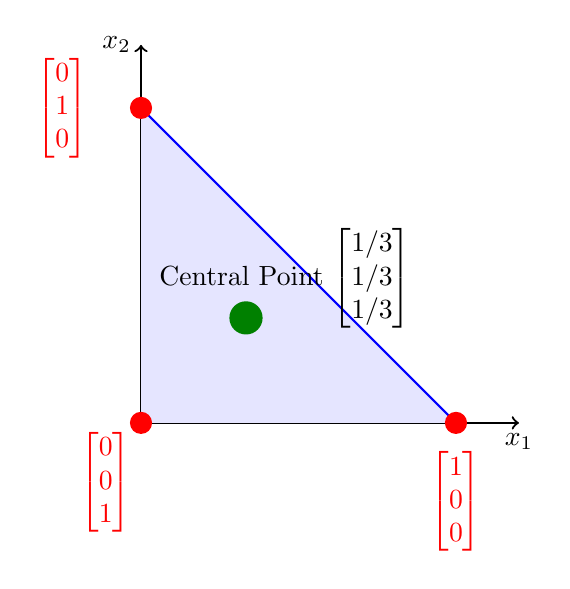
\begin{tikzpicture}[scale=4]
    % Axes
    \draw[->, thick] (0,0) -- (1.2,0) node[below] {$x_1$};
    \draw[->, thick] (0,0) -- (0,1.2) node[left] {$x_2$};

    % The projected simplex region (x1 + x2 <= 1)
    \fill[blue!10] (0,0) -- (1,0) -- (0,1) -- cycle;
    \draw[blue, thick] (1,0) -- (0,1);

    % The three vertices of the simplex
    \fill[red] (1,0) circle (1pt) node[shift={(0, -1)}] {$\begin{bmatrix} 1 \\ 0 \\ 0 \end{bmatrix}$};
    \fill[red] (0,1) circle (1pt) node[shift={(-1, 0)}] {$\begin{bmatrix} 0 \\ 1 \\ 0 \end{bmatrix}$};
    \fill[red] (0,0) circle (1pt) node[below left] {$\begin{bmatrix} 0 \\ 0 \\ 1 \end{bmatrix}$};

    % The central point (centroid)
    \fill[green!50!black] (1/3, 1/3) circle (1.5pt) node[shift={(0.5,0.5)}, black] {Central Point $\begin{bmatrix} 1/3 \\ 1/3 \\ 1/3 \end{bmatrix}$};
\end{tikzpicture}
\caption{View 1: Projection onto the $x_1$-$x_2$ plane.}
\label{fig:x1x2}
\end{figure}

%---------------------------------------------------
%  FIGURE 2: x2 vs x3 Projection
%---------------------------------------------------
\begin{figure}[h!]
\centering
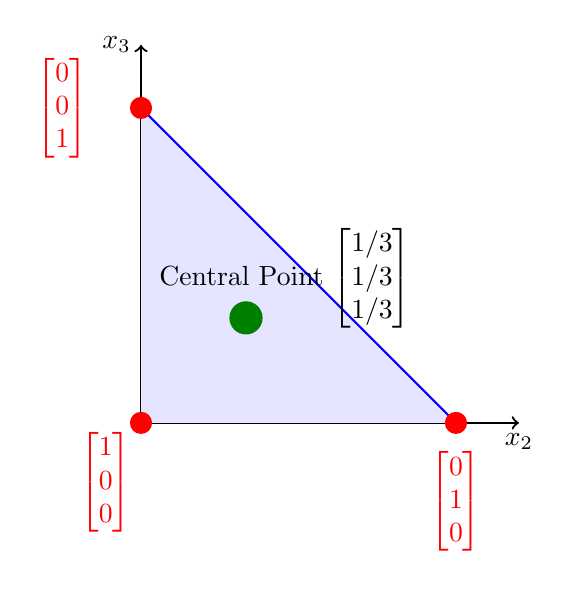
\begin{tikzpicture}[scale=4]
    % Axes
    \draw[->, thick] (0,0) -- (1.2,0) node[below] {$x_2$};
    \draw[->, thick] (0,0) -- (0,1.2) node[left] {$x_3$};

    % The projected simplex region (x2 + x3 <= 1)
    \fill[blue!10] (0,0) -- (1,0) -- (0,1) -- cycle;
    \draw[blue, thick] (1,0) -- (0,1);

    % The three vertices of the simplex
    \fill[red] (1,0) circle (1pt) node[shift={(0, -1)}] {$\begin{bmatrix} 0 \\ 1 \\ 0 \end{bmatrix}$};
    \fill[red] (0,1) circle (1pt) node[shift={(-1, 0)}] {$\begin{bmatrix} 0 \\ 0 \\ 1 \end{bmatrix}$};
    \fill[red] (0,0) circle (1pt) node[below left] {$\begin{bmatrix} 1 \\ 0 \\ 0 \end{bmatrix}$};

    % The central point (centroid)
    \fill[green!50!black] (1/3, 1/3) circle (1.5pt) node[shift={(0.5,0.5)}, black] {Central Point $\begin{bmatrix} 1/3 \\ 1/3 \\ 1/3 \end{bmatrix}$};
\end{tikzpicture}
\caption{View 2: Projection onto the $x_2$-$x_3$ plane.}
\label{fig:x2x3}
\end{figure}

\newpage

\subsection*{Solution 5}
\noindent\rule{\textwidth}{0.4pt}\\
%---------------------------------------------------
%  FIGURE 3: x1 vs x3 Projection
%---------------------------------------------------
\begin{figure}[h!]
\centering
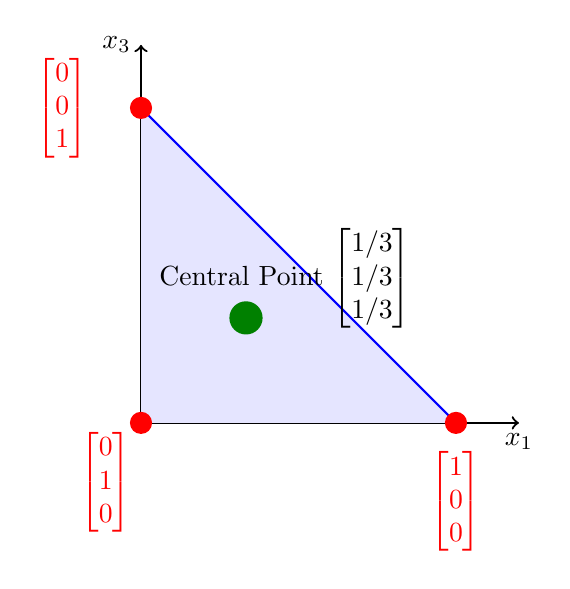
\begin{tikzpicture}[scale=4]
    % Axes
    \draw[->, thick] (0,0) -- (1.2,0) node[below] {$x_1$};
    \draw[->, thick] (0,0) -- (0,1.2) node[left] {$x_3$};

    % The projected simplex region (x1 + x3 <= 1)
    \fill[blue!10] (0,0) -- (1,0) -- (0,1) -- cycle;
    \draw[blue, thick] (1,0) -- (0,1);

    % The three vertices of the simplex
    \fill[red] (1,0) circle (1pt) node[shift={(0, -1)}] {$\begin{bmatrix} 1 \\ 0 \\ 0 \end{bmatrix}$};
    \fill[red] (0,1) circle (1pt) node[shift={(-1, 0)}] {$\begin{bmatrix} 0 \\ 0 \\ 1 \end{bmatrix}$};
    \fill[red] (0,0) circle (1pt) node[below left] {$\begin{bmatrix} 0 \\ 1 \\ 0 \end{bmatrix}$};

    % The central point (centroid)
    \fill[green!50!black] (1/3, 1/3) circle (1.5pt) node[shift={(0.5,0.5)}, black] {Central Point $\begin{bmatrix} 1/3 \\ 1/3 \\ 1/3 \end{bmatrix}$};
\end{tikzpicture}
\caption{View 3: Projection onto the $x_1$-$x_3$ plane.}
\label{fig:x1x3}
\end{figure}

\noindent\rule{\textwidth}{0.4pt}\\

\newpage

%------------------
% Solution for 6
%------------------
\subsection*{Solution 6}
\noindent\rule{\textwidth}{0.4pt}\\

\subsubsection*{Step 1: Recall the formulas for $\ell_1$ distance and KL divergence}
\parbox{\textwidth}{
    IDK.. LOG IS BASE e NOT 2
The $\ell_1$ distance (Manhattan distance) between two vectors $u$ and $v$ is:
$$\|u - v\|_1 = \sum_{i=1}^{n} |u_i - v_i|$$

The KL divergence between two probability distributions $P$ and $Q$ is:
$$KL(P \| Q) = \sum_{i=1}^{n} P_i \log\left(\frac{P_i}{Q_i}\right)$$
where we use the convention that $0 \log(0/Q_i) = 0$ and $P_i \log(P_i/0) = \infty$ if $P_i > 0$.
}

\subsubsection*{Step 2: Calculate each distance and divergence}
\parbox{\textwidth}{
\textbf{Part (i):} $\|p - q\|_1$ where $p = \begin{bmatrix} 1/2 \\ 1/4 \\ 1/8 \\ 1/8 \end{bmatrix}$ and $q = \begin{bmatrix} 1/4 \\ 1/4 \\ 1/4 \\ 1/4 \end{bmatrix}$

$$p - q = \begin{bmatrix} 1/2 - 1/4 \\ 1/4 - 1/4 \\ 1/8 - 1/4 \\ 1/8 - 1/4 \end{bmatrix} = \begin{bmatrix} 1/4 \\ 0 \\ -1/8 \\ -1/8 \end{bmatrix}$$

$$\|p - q\|_1 = |1/4| + |0| + |-1/8| + |-1/8| = 1/4 + 0 + 1/8 + 1/8 = 1/4 + 1/4 = 1/2$$

\textbf{Part (ii):} $\|q - r\|_1$ where $q = \begin{bmatrix} 1/4 \\ 1/4 \\ 1/4 \\ 1/4 \end{bmatrix}$ and $r = \begin{bmatrix} 1/2 \\ 0 \\ 1/4 \\ 1/4 \end{bmatrix}$

$$q - r = \begin{bmatrix} 1/4 - 1/2 \\ 1/4 - 0 \\ 1/4 - 1/4 \\ 1/4 - 1/4 \end{bmatrix} = \begin{bmatrix} -1/4 \\ 1/4 \\ 0 \\ 0 \end{bmatrix}$$

$$\|q - r\|_1 = |-1/4| + |1/4| + |0| + |0| = 1/4 + 1/4 + 0 + 0 = 1/2$$

\textbf{Part (iii):} $KL(p \| q)$

$$KL(p \| q) = \sum_{i=1}^{4} p_i \log\left(\frac{p_i}{q_i}\right)$$
$$= \frac{1}{2}\log\left(\frac{1/2}{1/4}\right) + \frac{1}{4}\log\left(\frac{1/4}{1/4}\right) + \frac{1}{8}\log\left(\frac{1/8}{1/4}\right) + \frac{1}{8}\log\left(\frac{1/8}{1/4}\right)$$
$$= \frac{1}{2}\log(2) + \frac{1}{4}\log(1) + \frac{1}{8}\log(1/2) + \frac{1}{8}\log(1/2)$$
$$= \frac{1}{2}\log(2) + 0 + \frac{1}{8}(-\log(2)) + \frac{1}{8}(-\log(2))$$
$$= \frac{1}{2}\log(2) - \frac{1}{4}\log(2) = \frac{1}{4}\log(2)$$

\textbf{Part (iv):} $KL(q \| r)$

$$KL(q \| r) = \sum_{i=1}^{4} q_i \log\left(\frac{q_i}{r_i}\right)$$
$$= \frac{1}{4}\log\left(\frac{1/4}{1/2}\right) + \frac{1}{4}\log\left(\frac{1/4}{0}\right) + \frac{1}{4}\log\left(\frac{1/4}{1/4}\right) + \frac{1}{4}\log\left(\frac{1/4}{1/4}\right)$$

Since $r_2 = 0$ and $q_2 = 1/4 > 0$, we have $\log(q_2/r_2) = \log(1/4/0) = +\infty$.

Therefore: $KL(q \| r) = +\infty$
}

\subsubsection*{\normalfont}{$\therefore$ Final Answers}
\begin{enumerate}
\item $\|p - q\|_1 = \frac{1}{2}$
\item $\|q - r\|_1 = \frac{1}{2}$
\item $KL(p \| q) = \frac{1}{4}\log(2) \approx 0.173$
\item $KL(q \| r) = +\infty$
\end{enumerate}

\subsubsection*{\normalfont}{Graduate Level Explanation}
The $\ell_1$ distance is symmetric and satisfies the triangle inequality, making it a proper metric on the probability simplex. Interestingly, both pairs have the same $\ell_1$ distance despite having different structures. The KL divergence, however, is asymmetric and not a true metric. $KL(p \| q)$ is finite because $q$ has full support (no zero entries), but $KL(q \| r) = \infty$ because $r$ has a zero entry where $q$ has positive probability. This illustrates a fundamental property: KL divergence from a distribution with full support to one with restricted support is infinite, making it useful for detecting when probability mass is assigned to impossible events in the reference distribution.

\subsubsection*{\normalfont}{Explanation for 5 year old}
The $\ell_1$ distance is like counting how much you need to move marbles between jars to make them the same - it's always the same no matter which direction you go. But KL divergence is like asking "how surprised would I be?" If one jar is completely empty but you expected marbles there, you'd be infinitely surprised! That's why one answer is infinity - it's like expecting something that's impossible.

\noindent\rule{\textwidth}{0.4pt}\\

\newpage
%------------------
% Solution for 7
%------------------
\subsection*{Solution 7}
\noindent\rule{\textwidth}{0.4pt}\\
\subsubsection*{Part a: Dimensionality for each of the representations (raw pixel, HoG, VGG-last-fc, VGG-last-conv)}
\begin{center} 
  \begin{tabular}{|c|c|} 
    \hline Feature Type & Dimensionality \\ 
    \hline 
    Raw Pixel & 3072 \\ 
    HoG & 512  \\
    VGG-last-fc & 4096 \\
    VGG-last-conv & 512 \\ 
    \hline
  \end{tabular}
\end{center}

\noindent\rule{\textwidth}{0.4pt}\\

\subsubsection*{Part b: Test accuracies for 1-nearest neighbor classification using the various representations (raw pixel, HoG, VGG-last-fc, VGG-last-conv, random-VGG-last-fc, random-VGG-last-conv).}
\begin{center} 
  \begin{tabular}{|c|c|} 
    \hline Feature Type & 1-NN test accuracy (\%) \\ 
    \hline 
    Raw Pixel & 35.4 \\ 
    HoG & 36.6  \\
    VGG-last-fc & 92.1 \\
    VGG-last-conv & 92.0 \\
    random VGG-last-fc & 39.1 \\
    random VGG-last-conv & 40.6 \\ 
    \hline
  \end{tabular}
\end{center}
\noindent\rule{\textwidth}{0.4pt}\\

\newpage

\subsection*{Solution 7}
\noindent\rule{\textwidth}{0.4pt}\\
\subsubsection*{Part c:  Raw Pixel correct/incorrect}

\begin{figure}[h]
  \includegraphics[height=0.75\textheight,width=\textwidth]{raw_pixel.png}
  \caption{First five correct/incorrect images for Raw Pixel}
\end{figure}

\newpage

\subsection*{Solution 7}
\noindent\rule{\textwidth}{0.4pt}\\
\subsubsection*{Part c:  HoG correct/incorrect}

\begin{figure}[h]
  \includegraphics[height=0.75\textheight,width=\textwidth]{hog.png}
  \caption{First five correct/incorrect images for HoG}
\end{figure}

\newpage

\subsection*{Solution 7}
\noindent\rule{\textwidth}{0.4pt}\\
\subsubsection*{Part c:  VGG-last-fc correct/incorrect}

\begin{figure}[h]
  \includegraphics[height=0.75\textheight,width=\textwidth]{vgg_last_fc.png}
  \caption{First five correct/incorrect images for VGG-last-fc}
\end{figure}

\newpage

\subsection*{Solution 8}
\noindent\rule{\textwidth}{0.4pt}\\
\subsubsection*{Word Vectors: 5 closest words}
\begin{center} 
  \begin{tabular}{|c|c|} 
    \hline Target Word & Five Closest Words \\ 
    \hline 
    communism & \text{['fascism', 'capitalism', 'nazism', 'stalinism', 'socialism']} \\ 
    africa & \text{['african', 'continent', 'south', 'africans', 'zimbabwe']}  \\
    happy & \text{['glad', 'pleased', 'always', 'everyone', 'sure']} \\
    sad & \text{['sorry', 'tragic', 'happy', 'pathetic', 'awful']} \\ 
    upset & \text{['upsetting', 'surprised', 'upsets', 'stunned', 'shocked']}\\
    computer & \text{['computers', 'software', 'technology', 'laptop', 'computing']}\\
    cat & \text{['cats', 'dog', 'pet', 'feline', 'dogs']}\\
    dollar & \text{['currency', 'dollars', 'euro', 'multibillion', 'weaker']}\\

    \hline
  \end{tabular}
\end{center}

\noindent\rule{\textwidth}{0.4pt}\\

% raw_acc: 35.4%
% hog_acc: 36.6%
% pretrain_cnn_acc(last_conv): 92.0%
% pretrain_cnn_acc(last_fc): 92.1%
% random_cnn_acc(last_conv): 40.6%
% random_cnn_acc(last_fc): 39.1%

\newpage

\subsection*{Solution 1: Scalability on the Probability Simplex}

\subsubsection*{Step 1: Define the Probability Simplex $\Delta_2$}
\parbox{\textwidth}{
  The probability simplex $\Delta_k$ is the set of all $k$-dimensional vectors with non-negative components that sum to 1. For $k=2$, a vector $p = \begin{bmatrix} p_1 \\ p_2 \end{bmatrix}$ is in $\Delta_2$ if and only if it satisfies two conditions:
\begin{enumerate}
    \item \textbf{Non-negativity:} $p_1 \geq 0$ and $p_2 \geq 0$.
    \item \textbf{Sum-to-one:} $p_1 + p_2 = 1$.
\end{enumerate}
The question asks if for any vector $p \in \mathbb{R}^2$ and scalar $c > 0$, the condition $c \cdot p \in \Delta_2$ implies that $p \in \Delta_2$.}

\subsubsection*{Step 2: Analyze the Constraints under Scaling}
\parbox{\textwidth}{Let $q = c \cdot p = \begin{bmatrix} c p_1 \\ c p_2 \end{bmatrix}$. We are given that $q \in \Delta_2$.
\begin{itemize}
    \item \textbf{Non-negativity:} Since $c > 0$ and we are given $c p_1 \geq 0$ and $c p_2 \geq 0$, it must be that $p_1 \geq 0$ and $p_2 \geq 0$. This condition is satisfied for $p$.
    \item \textbf{Sum-to-one:} We are given that the components of $q$ sum to 1: $c p_1 + c p_2 = 1$. Factoring out $c$, we get $c(p_1 + p_2) = 1$, which implies $p_1 + p_2 = \frac{1}{c}$.
\end{itemize}
For $p$ to be in $\Delta_2$, its components must sum to 1, i.e., $p_1 + p_2 = 1$. This only holds if $\frac{1}{c} = 1$, which means $c=1$. Since the statement must hold for any $c > 0$, we can find a counterexample by choosing $c \neq 1$.}

\subsubsection*{Step 3: Construct a Counterexample}
\parbox{\textwidth}{Let $c=2$. Choose a point $q \in \Delta_2$, for example, $q = \begin{bmatrix} 0.5 \\ 0.5 \end{bmatrix}$.
If $c \cdot p = q$, then $p = \frac{1}{c} q = \frac{1}{2} \begin{bmatrix} 0.5 \\ 0.5 \end{bmatrix} = \begin{bmatrix} 0.25 \\ 0.25 \end{bmatrix}$.
Let's check if this $p$ is in $\Delta_2$:
\begin{itemize}
    \item \textbf{Non-negativity:} $p_1 = 0.25 \geq 0$ and $p_2 = 0.25 \geq 0$. (Satisfied)
    \item \textbf{Sum-to-one:} $p_1 + p_2 = 0.25 + 0.25 = 0.5 \neq 1$. (Not satisfied)
\end{itemize}
Since $p$ does not satisfy the sum-to-one constraint, $p \notin \Delta_2$. Thus, the statement is false.}

\subsubsection*{\normalfont}{$\therefore$ Final Answer}\\
\parbox{\textwidth}{The statement is \textbf{false}. A counterexample is $p = \begin{bmatrix} 0.25 \\ 0.25 \end{bmatrix}$ and $c=2$. Here, $c \cdot p = \begin{bmatrix} 0.5 \\ 0.5 \end{bmatrix} \in \Delta_2$, but $p \notin \Delta_2$ because its components sum to $0.5$, not $1$.}

\subsubsection*{\normalfont}{Graduate Level Explanation}\\
\parbox{\textwidth}{
  The probability simplex $\Delta_k$ is an affine subspace of $\mathbb{R}^k$, specifically the intersection of the hyperplane $\sum x_i = 1$ and the non-negative orthant $\mathbb{R}^k_+$. While the non-negative orthant is a convex cone (closed under non-negative scalar multiplication), the hyperplane $\sum x_i = 1$ is not a linear subspace as it does not contain the origin. Scaling a vector $p$ by $c \neq 1$ moves it off this hyperplane, thus violating the sum-to-one constraint. The set of vectors whose scaled versions lie on the simplex forms a cone over the simplex, but these vectors are not, in general, on the simplex themselves.}

\subsubsection*{\normalfont}{Explanation for a 5 year old}\\
\parbox{\textwidth}{Imagine a recipe for one special juice drink says you need 1 cup of ingredients in total. This "1 cup total" rule is very important. You find a bottle of juice that follows the rule. Your friend says, "I have a different bottle, and if I pour out half of it, it's exactly the same as your juice." Your friend's bottle might follow the non-negativity rule (it has juice in it), but it must have had 2 cups of ingredients to begin with. So, your friend's original bottle did not follow the "1 cup total" rule.}

\noindent\rule{\textwidth}{0.4pt}\\\\

\subsection*{Solution 2: Sketching the Probability Simplex $\Delta_3$}

\subsubsection*{Step 1: Define the Geometry of $\Delta_3$}
\parbox{\textwidth}{The probability simplex $\Delta_3$ is the set of points $p = \begin{bmatrix} p_1 & p_2 & p_3 \end{bmatrix}^\top$ in $\mathbb{R}^3$ satisfying:
\begin{enumerate}
    \item $p_1 \geq 0, p_2 \geq 0, p_3 \geq 0$ (it lies in the first octant).
    \item $p_1 + p_2 + p_3 = 1$ (it lies on a plane).
\end{enumerate}
The intersection of the plane $p_1+p_2+p_3=1$ with the first octant forms a bounded, closed shape. To identify the shape, we find its vertices.}

\subsubsection*{Step 2: Identify the Vertices and the Central Point}
\parbox{\textwidth}{The vertices of the shape are the points where the plane intersects the coordinate axes.
\begin{itemize}
    \item Intersection with $p_1$-axis ($p_2=0, p_3=0$): $p_1 = 1$. Vertex $v_1 = \begin{bmatrix} 1 & 0 & 0 \end{bmatrix}^\top$.
    \item Intersection with $p_2$-axis ($p_1=0, p_3=0$): $p_2 = 1$. Vertex $v_2 = \begin{bmatrix} 0 & 1 & 0 \end{bmatrix}^\top$.
    \item Intersection with $p_3$-axis ($p_1=0, p_2=0$): $p_3 = 1$. Vertex $v_3 = \begin{bmatrix} 0 & 0 & 1 \end{bmatrix}^\top$.
\end{itemize}
Connecting these three vertices in 3D space forms an equilateral triangle. The "most central" point of this triangle is its barycenter (or centroid), which is the average of the coordinates of its vertices.}

\subsubsection*{Step 3: Calculate the Centroid}
\parbox{\textwidth}{The coordinates of the centroid $p_c$ are:
$$ p_c = \frac{v_1 + v_2 + v_3}{3} = \frac{1}{3} \left( \begin{bmatrix} 1 \\ 0 \\ 0 \end{bmatrix} + \begin{bmatrix} 0 \\ 1 \\ 0 \end{bmatrix} + \begin{bmatrix} 0 \\ 0 \\ 1 \end{bmatrix} \right) = \frac{1}{3} \begin{bmatrix} 1 \\ 1 \\ 1 \end{bmatrix} = \begin{bmatrix} 1/3 \\ 1/3 \\ 1/3 \end{bmatrix} $$
This point corresponds to the uniform probability distribution over three outcomes.}

\subsubsection*{\normalfont}{$\therefore$ Final Answer}\\
\parbox{\textwidth}{\textbf{Sketch Description:} The probability simplex $\Delta_3$ is an equilateral triangle in 3D space whose vertices are at the standard basis vectors $\begin{bmatrix} 1, 0, 0 \end{bmatrix}^\top$, $\begin{bmatrix} 0, 1, 0 \end{bmatrix}^\top$, and $\begin{bmatrix} 0, 0, 1 \end{bmatrix}^\top$.

\textbf{Most Central Point:} The coordinates of the most central point (the barycenter) are $\begin{bmatrix} 1/3 \\ 1/3 \\ 1/3 \end{bmatrix}^\top$.}

\subsubsection*{\normalfont}{Graduate Level Explanation}\\
\parbox{\textwidth}{The standard $k$-simplex, $\Delta_k$, is a $(k-1)$-dimensional convex polytope embedded in $\mathbb{R}^k$. For $k=3$, this results in a 2-dimensional triangle. The vertices are the standard basis vectors $e_1, e_2, e_3$, representing deterministic probability distributions. The barycenter of the simplex, $(1/k, \dots, 1/k)^\top$, corresponds to the uniform probability distribution. In information theory, this is the distribution with the maximum Shannon entropy, representing the state of maximum uncertainty.}

\subsubsection*{\normalfont}{Explanation for a 5 year old}\\
\parbox{\textwidth}{Imagine a big glass cube. Now, imagine you slice it with a flat piece of glass. The slice starts at the number 1 on the `x` line, goes to the number 1 on the `y` line, and also to the number 1 on the `z` line. The shape of this flat slice inside the corner of the cube is a perfect triangle. The very middle of that triangle is its balancing point. That special point is at $(1/3, 1/3, 1/3)$, which means it's an equal distance from all three number lines.}

\noindent\rule{\textwidth}{0.4pt}\\\\

\subsection*{Solution 3: $\ell_1$ Distance and KL Divergence}

\subsubsection*{Step 1: Calculate the $\ell_1$ Distance}
\parbox{\textwidth}{The $\ell_1$ distance between two vectors $p, q \in \mathbb{R}^n$ is given by $\|p-q\|_1 = \sum_{i=1}^n |p_i - q_i|$.
For $p = \begin{bmatrix} 1/2 & 1/4 & 1/8 & 1/8 \end{bmatrix}^\top$ and $q = \begin{bmatrix} 1/4 & 1/4 & 1/4 & 1/4 \end{bmatrix}^\top$:
\begin{align*}
    \|p-q\|_1 &= \left|\frac{1}{2} - \frac{1}{4}\right| + \left|\frac{1}{4} - \frac{1}{4}\right| + \left|\frac{1}{8} - \frac{1}{4}\right| + \left|\frac{1}{8} - \frac{1}{4}\right| \\
    &= \left|\frac{2}{4} - \frac{1}{4}\right| + |0| + \left|\frac{1}{8} - \frac{2}{8}\right| + \left|\frac{1}{8} - \frac{2}{8}\right| \\
    &= \frac{1}{4} + 0 + \left|-\frac{1}{8}\right| + \left|-\frac{1}{8}\right| \\
    &= \frac{1}{4} + \frac{1}{8} + \frac{1}{8} = \frac{2}{8} + \frac{1}{8} + \frac{1}{8} = \frac{4}{8} = \frac{1}{2}
\end{align*}}

\subsubsection*{Step 2: Calculate the KL Divergence $K(p, q)$}
\parbox{\textwidth}{The Kullback-Leibler (KL) divergence from $q$ to $p$ is $K(p, q) = \sum_{i=1}^n p_i \ln \frac{p_i}{q_i}$.
\begin{align*}
    K(p, q) &= p_1 \ln\left(\frac{p_1}{q_1}\right) + p_2 \ln\left(\frac{p_2}{q_2}\right) + p_3 \ln\left(\frac{p_3}{q_3}\right) + p_4 \ln\left(\frac{p_4}{q_4}\right) \\
    &= \frac{1}{2} \ln\left(\frac{1/2}{1/4}\right) + \frac{1}{4} \ln\left(\frac{1/4}{1/4}\right) + \frac{1}{8} \ln\left(\frac{1/8}{1/4}\right) + \frac{1}{8} \ln\left(\frac{1/8}{1/4}\right) \\
    &= \frac{1}{2} \ln(2) + \frac{1}{4} \ln(1) + \frac{1}{8} \ln\left(\frac{1}{2}\right) + \frac{1}{8} \ln\left(\frac{1}{2}\right) \\
    &= \frac{1}{2} \ln(2) + 0 - \frac{1}{8} \ln(2) - \frac{1}{8} \ln(2) \\
    &= \left(\frac{1}{2} - \frac{1}{8} - \frac{1}{8}\right) \ln(2) = \left(\frac{4}{8} - \frac{2}{8}\right) \ln(2) = \frac{2}{8} \ln(2) = \frac{1}{4} \ln(2)
\end{align*}}

\subsubsection*{Step 3: Calculate the KL Divergence $K(q, p)$}
\parbox{\textwidth}{The KL divergence from $p$ to $q$ is $K(q, p) = \sum_{i=1}^n q_i \ln \frac{q_i}{p_i}$.
\begin{align*}
    K(q, p) &= q_1 \ln\left(\frac{q_1}{p_1}\right) + q_2 \ln\left(\frac{q_2}{p_2}\right) + q_3 \ln\left(\frac{q_3}{p_3}\right) + q_4 \ln\left(\frac{q_4}{p_4}\right) \\
    &= \frac{1}{4} \ln\left(\frac{1/4}{1/2}\right) + \frac{1}{4} \ln\left(\frac{1/4}{1/4}\right) + \frac{1}{4} \ln\left(\frac{1/4}{1/8}\right) + \frac{1}{4} \ln\left(\frac{1/4}{1/8}\right) \\
    &= \frac{1}{4} \ln\left(\frac{1}{2}\right) + \frac{1}{4} \ln(1) + \frac{1}{4} \ln(2) + \frac{1}{4} \ln(2) \\
    &= -\frac{1}{4} \ln(2) + 0 + \frac{1}{4} \ln(2) + \frac{1}{4} \ln(2) \\
    &= \frac{1}{4} \ln(2)
\end{align*}}

\subsubsection*{\normalfont}{$\therefore$ Final Answer}\\
\parbox{\textwidth}{For the given probability distributions $p$ and $q$:
\begin{itemize}
    \item The $\ell_1$ distance is $\|p-q\|_1 = \mathbf{\frac{1}{2}}$.
    \item The KL divergence from $q$ to $p$ is $K(p, q) = \mathbf{\frac{1}{4} \ln(2)}$.
    \item The KL divergence from $p$ to $q$ is $K(q, p) = \mathbf{\frac{1}{4} \ln(2)}$.
\end{itemize}}

\subsubsection*{\normalfont}{Graduate Level Explanation}\\
\parbox{\textwidth}{The $\ell_1$ distance is a true metric satisfying symmetry and the triangle inequality; on the probability simplex, it is equivalent to twice the total variation distance. The Kullback-Leibler divergence, conversely, is not a metric. It is asymmetric ($K(p,q) \neq K(q,p)$ in general, although they coincide in this specific case) and does not satisfy the triangle inequality. It is a Bregman divergence generated by the negative entropy function, and it quantifies the expected inefficiency (in terms of information) of using a code optimized for distribution $q$ to encode data from the true distribution $p$. By Gibbs' inequality, $K(p,q) \geq 0$ with equality if and only if $p=q$.}

\subsubsection*{\normalfont}{Explanation for a 5 year old}\\
\parbox{\textwidth}{\textbf{L1 Distance:} Imagine you have two towers built from 4 kinds of colored blocks. Tower P has 4 red, 2 blue, 1 green, 1 yellow. Tower Q has 2 red, 2 blue, 2 green, 2 yellow. The "distance" is how many blocks you have to move to make Tower P look exactly like Tower Q. You need to take 2 red blocks away and add 1 green and 1 yellow. That's 4 moves in total. Our math gives an answer of 1/2, which is like a grown-up way of counting this.

\textbf{KL Divergence:} This is like a guessing game. Your bag of marbles has the colors mixed like in Tower P. Your friend thinks the colors are mixed like in Tower Q. The KL number measures how "surprised" your friend will be, on average, each time they pull a marble from your bag. A bigger number means more surprise! It's not usually the same amount of surprise as if you pulled from their bag, but for these special towers, it happens to be the same.}

\end{document}


\end{document}